
\documentclass{beamer}

\usepackage{hyperref}
\usepackage[T1]{fontenc}
\usepackage{ctex}
\usepackage{tikz}
\definecolor{kvblue}{RGB}{12,74,133}
\UseRawInputEncoding

% Original packages
\usepackage{pgfpages}
\usepackage{latexsym,amsmath,xcolor,multicol,booktabs,calligra}
\usepackage{graphicx,listings,stackengine}

% =====================================
% Presentation Information
% =====================================

\title{Dropping Subword KV Entries After Detokenization}

\author[EE599 | Project Proposal]{
    \footnotesize
    Mahdi Heidari \quad | \quad
    Mohammad Mahdi Razmjoo \quad | \quad
    Amirreza Valaei \\
    Group 2
}

\institute[KAIST]{
    Large-Scale Foundation Models: Theory and Practice\\
    Instructor: Prof. Insu Han\\
}

\date{October 2026}

% Original theme
\usepackage{YTU}

\usepackage[backend=biber,style=authoryear,maxbibnames=3,maxcitenames=2,giveninits=true]{biblatex}
\addbibresource{refs.bib}
\begin{document}

% =====================================
% Slide 1: Original Title Page
% =====================================
\begin{frame}

    \titlepage

    \begin{figure}[htpb]
        \begin{center}
            
\includegraphics[width=0.2\linewidth]{pic/KAIST.png}
        \end{center}
    \end{figure}

\end{frame}

% =====================================
% Slide 2: Empty
% =====================================

\begin{frame}{Motivation: The Cost of Token-Level Memory}

\small

% Main observation
\textbf{A single word may be split into multiple
subword tokens.}

\vspace{0.10cm}

Each token requires a separate KV-cache entry
at every Transformer layer.

% Main figure
\begin{center}
    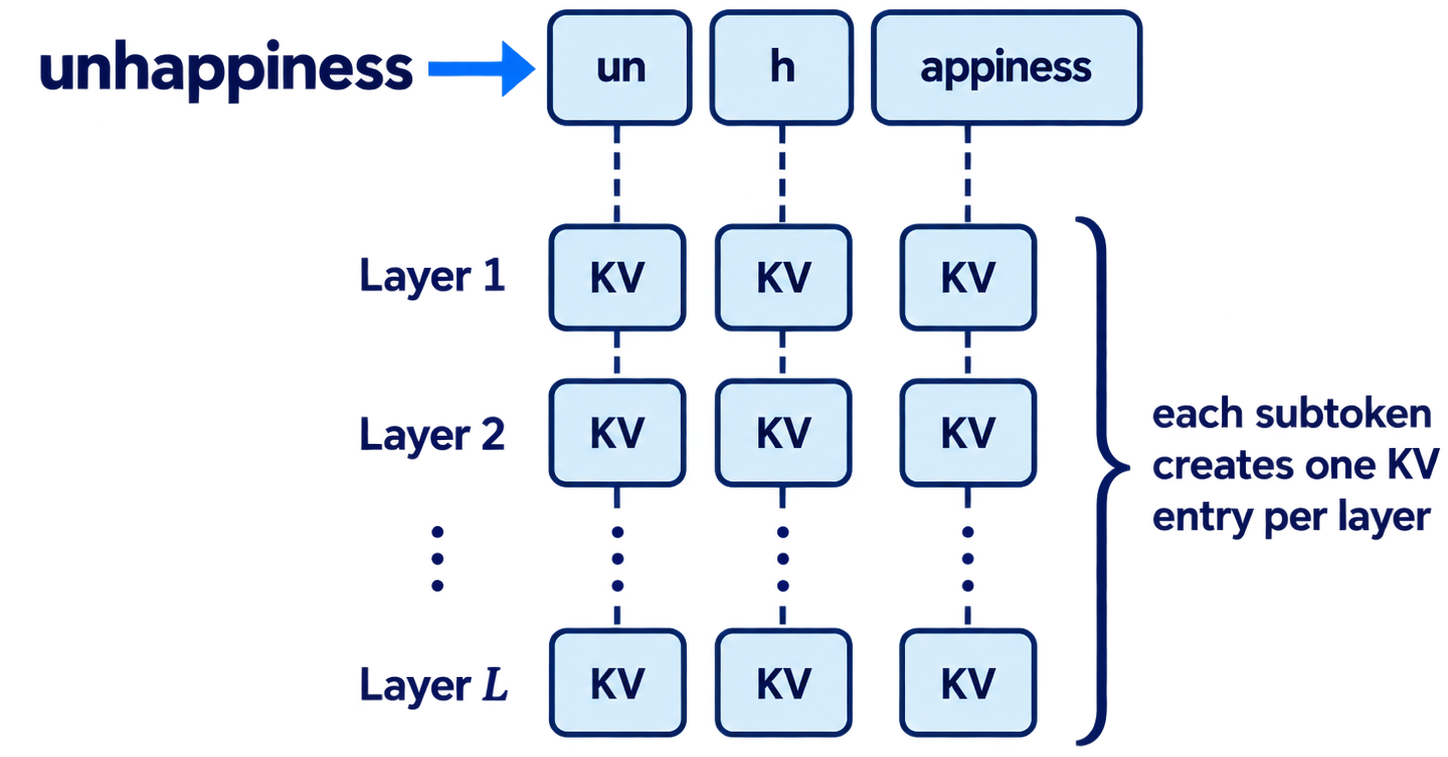
\includegraphics[
        width=0.8\linewidth,
        height=0.4\textheight,
        keepaspectratio
    ]{pic/img1.png}
\end{center}


% Research motivation
\pause
\centering
{\color{blue!65!black}
\textbf{Do we really need to keep all these
KV entries after processing the word?}
\par}

\end{frame}



% =====================================
% Slide 3: Prior Work
% =====================================
\begin{frame}{Prior Work: From Subtokens to Words}

\small

\textbf{LLMs reconstruct word-level information
at the final subtoken.}

\vspace{0.16cm}

\begin{columns}[T,onlytextwidth]

    % ============================
    % Left: Kaplan et al.
    % ============================
    \begin{column}{0.45\textwidth}
        \centering

        {\footnotesize\bfseries
        HOW: Attention + FFN\par}

        \vspace{0.10cm}

        \begin{minipage}[c][0.49\textheight][c]{\linewidth}
            \centering
            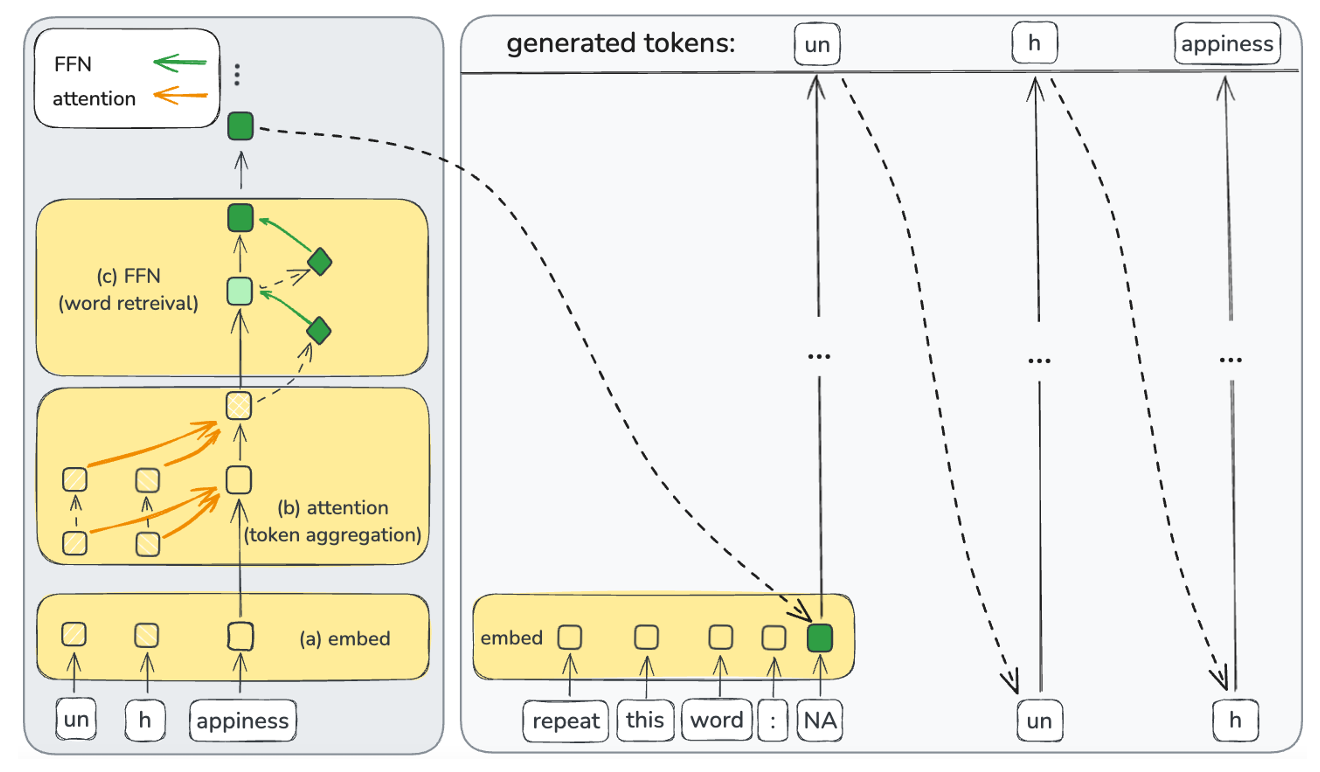
\includegraphics[
                width=0.94\linewidth,
                height=0.49\textheight,
                keepaspectratio
            ]{pic/img2.png}
        \end{minipage}

        \vspace{0.05cm}

        {\tiny From tokens to words: On the inner lexicon of LLMs \\
        \textcite{kaplan2025tokens}}

    \end{column}

    % ============================
    % Right: Busigin & Pinter
    % ============================
    \begin{column}{0.55\textwidth}
        \centering

        {\footnotesize\bfseries
        WHEN: Early layers\par}

        \vspace{0.10cm}

        \begin{minipage}[c][0.49\textheight][c]{\linewidth}
            \centering
            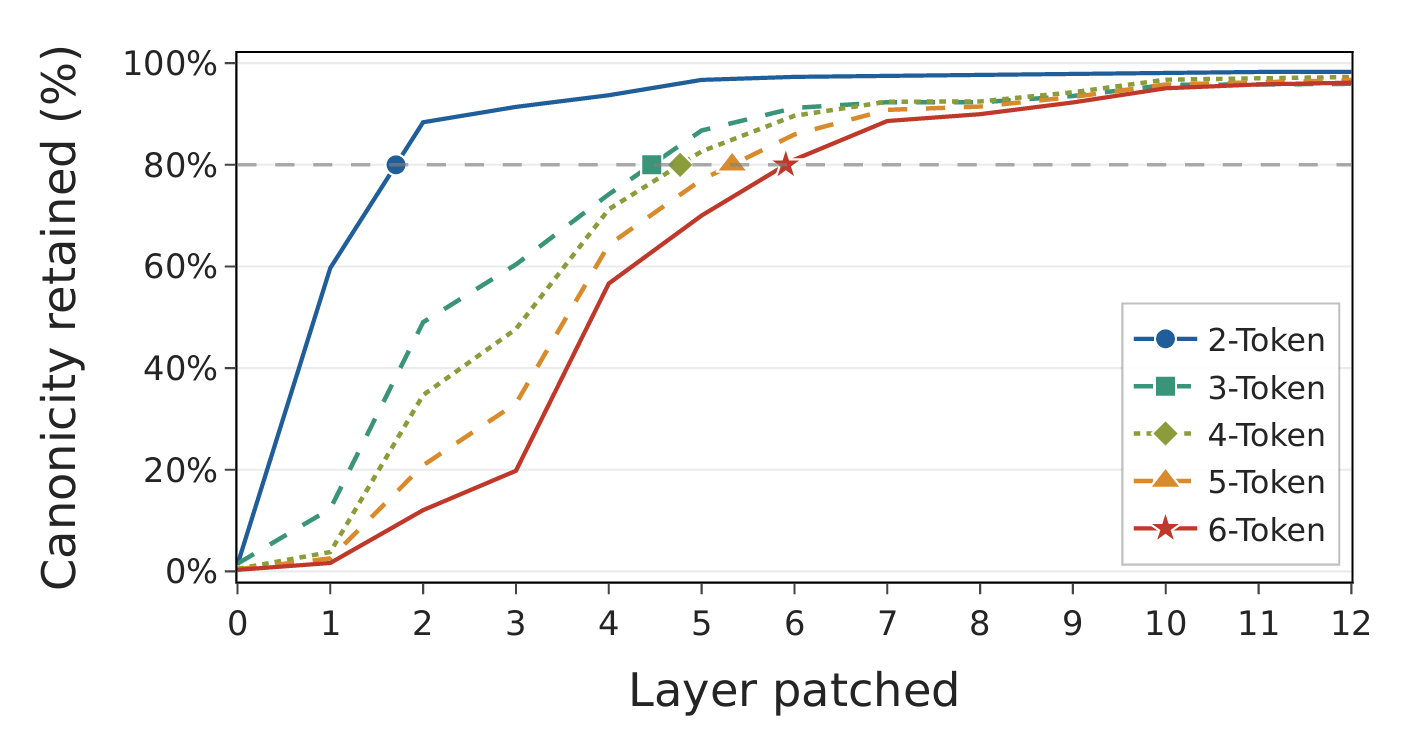
\includegraphics[
                width=\linewidth,
                height=0.49\textheight,
                keepaspectratio
            ]{pic/img3.png}
        \end{minipage}

        \vspace{0.05cm}

        {\tiny Inside the LLM Word Factory \\
        \textcite{busigin2026inside}}

    \end{column}

\end{columns}

\vspace{0.18cm}

\begin{center}
    {\footnotesize
    \color{blue!60!black}
    \bfseries
    Does this consolidation make earlier
    KV entries redundant?
    \par}
\end{center}

\end{frame}



\begin{frame}{Research Question \& Proposed Experiment}

\small

\textbf{Research Question:}
Can we discard / approximate earlier subtoken KV entries
after the word has been internally reconstructed?

\vspace{0.1cm}

\textbf{Intervention:}
After prefill, approximate non-final subtoken KV entries
from layer $s$ onward.

\vspace{0.05cm}

\begin{columns}[c,onlytextwidth]

    % ---------- Left: narrower, smaller text, vertically centred ----------
    \begin{column}{0.4\textwidth}
        \scriptsize
        \setlength{\topsep}{0pt}
        \setlength{\partopsep}{0pt}
        \setlength{\parsep}{0pt}
        \setlength{\parskip}{0pt}
        \begin{itemize}
            \setlength{\itemsep}{0.12cm}
            \item \textbf{Variants:} drop, merge into final subtoken, quantized.
            \item \textbf{Attention:} full, sparse, linear / hybrid.
        \end{itemize}
    \end{column}

    % ---------- Right: wider, bigger figure ----------
    \begin{column}{0.6\textwidth}
        \centering
        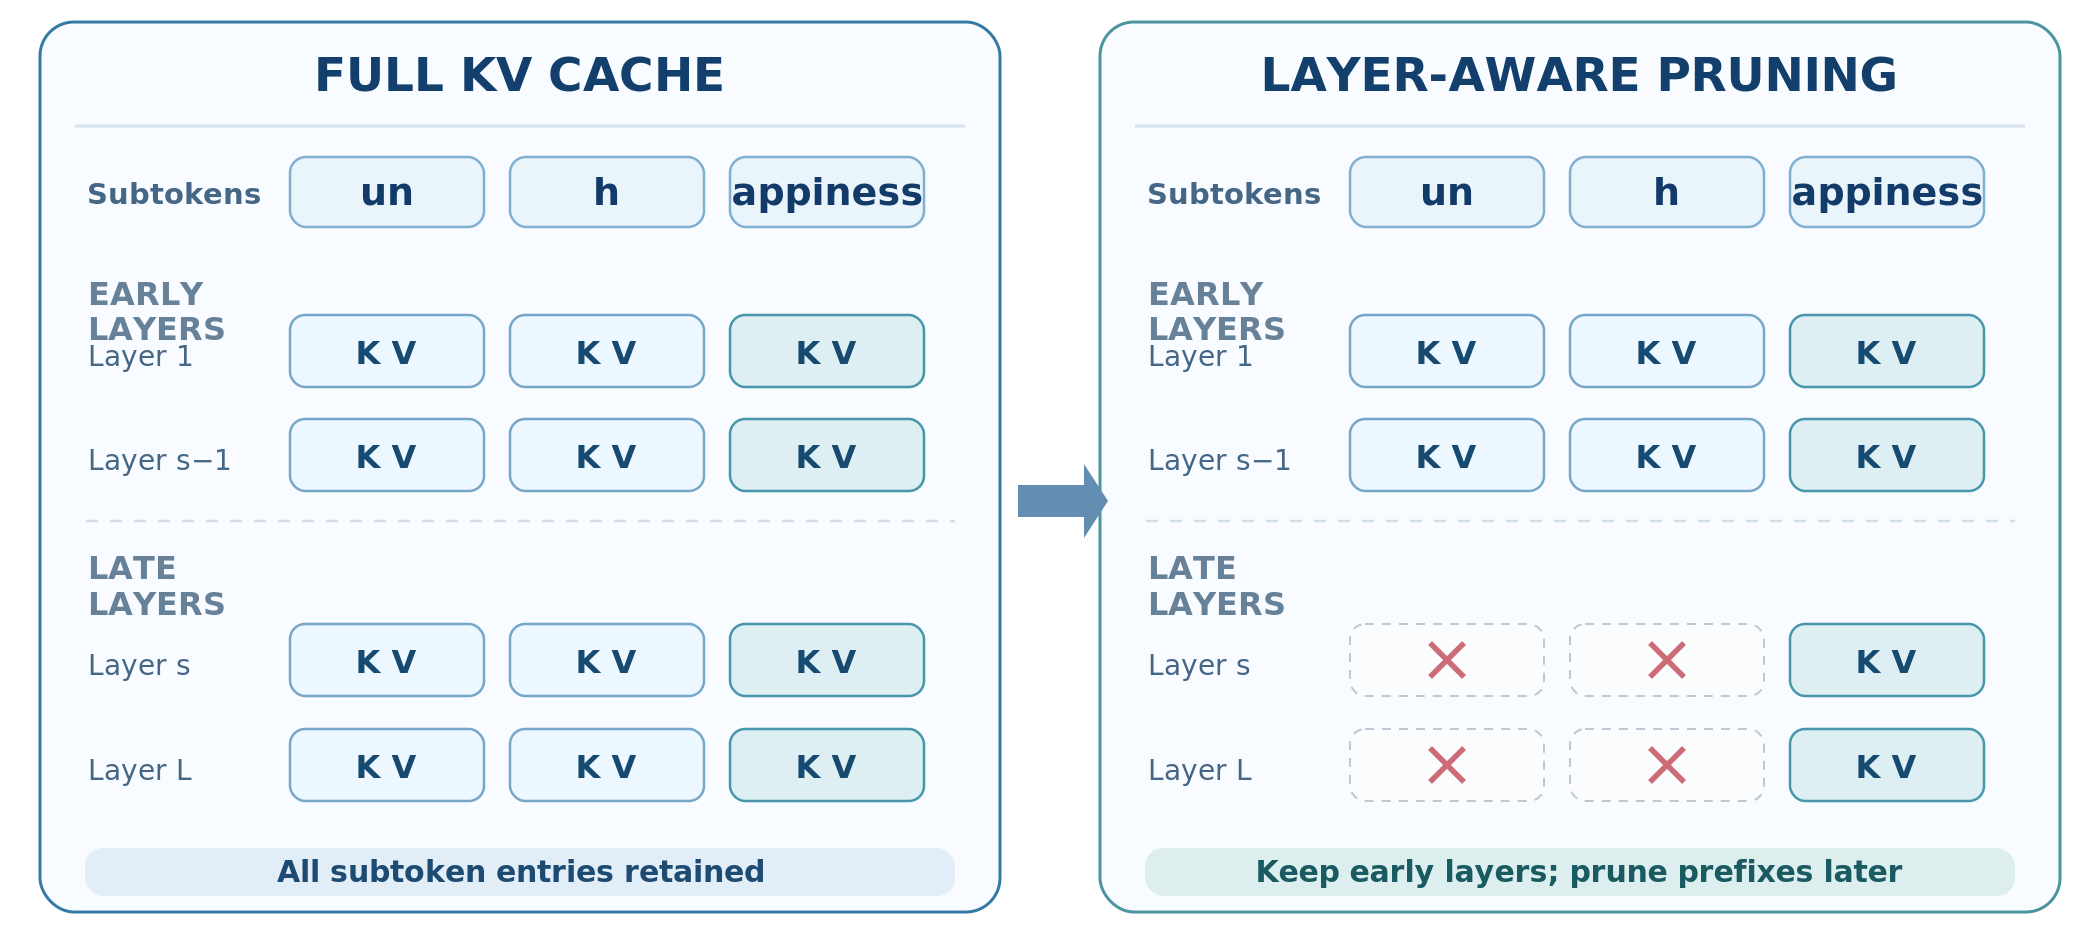
\includegraphics[
            width=\linewidth,
            height=0.58\textheight,
            keepaspectratio
        ]{pic/img4.png}
    \end{column}

\end{columns}

\vspace{0.05cm}

\textbf{Evaluation:}
Memory savings vs.\ quality degradation.

\vspace{0.1cm}
\pause
\begin{center}
    {\footnotesize
    \color{blue!65!black}
    \bfseries
    Hypothesis: Once the model has put the word together, the earlier KV entries are no longer needed.
    \par}
\end{center}

\end{frame}

\begin{frame}[allowframebreaks]{References}
    \footnotesize
    \printbibliography[heading=none]
\end{frame}


\end{document}
